\documentclass[12pt]{article}
\usepackage{fullpage}
\usepackage{url}
\usepackage{amsmath}
\usepackage{amsfonts}
\usepackage{algorithm}
\usepackage{algorithmic}
\usepackage{graphicx}
\usepackage{hyperref}
\usepackage{color}
\usepackage{listings}
\usepackage{verbatim}
\usepackage{enumitem}
\usepackage[parfill]{parskip}

\newcommand{\xb}{\mathbf{x}}
\newcommand{\yb}{\mathbf{y}}
\newcommand{\wb}{\mathbf{w}}
\newcommand{\Xb}{\mathbf{X}}
\newcommand{\Yb}{\mathbf{Y}}
\newcommand{\tr}{^T}
\newcommand{\hb}{\mathbf{h}}
\newcommand{\Hb}{\mathbf{H}}

\newcommand{\cmt}[1]{{\footnotesize\textcolor{red}{#1}}}
\newcommand{\todo}[1]{\cmt{TO-DO: #1}}

\title{CS294-112 Deep Reinforcement Learning HW3}

\author{ Heri Zhao
}

\date{Fall 2018}

\usepackage{courier}
 
\definecolor{codegreen}{rgb}{0,0.6,0}
\definecolor{codegray}{rgb}{0.5,0.5,0.5}
\definecolor{codepurple}{rgb}{0.58,0,0.82}
\definecolor{backcolour}{rgb}{0.95,0.95,0.92}

\lstdefinestyle{mystyle}{
    backgroundcolor=\color{backcolour},   
    commentstyle=\color{codegreen},
    keywordstyle=\color{magenta},
    numberstyle=\tiny\color{codegray},
    stringstyle=\color{codepurple},
    basicstyle=\footnotesize\ttfamily,
    breakatwhitespace=false,         
    breaklines=true,                 
    captionpos=b,                    
    keepspaces=true,                 
    %numbers=left,                    
    numbersep=5pt,                  
    showspaces=false,                
    showstringspaces=false,
    showtabs=false,                  
    tabsize=2
}

\lstset{style=mystyle}

\begin{document}

\maketitle

\section*{Part1 Q-learning}

\subsection*{Question 1: basic Q-learning performance}
\begin{figure}[H]
  \centering
  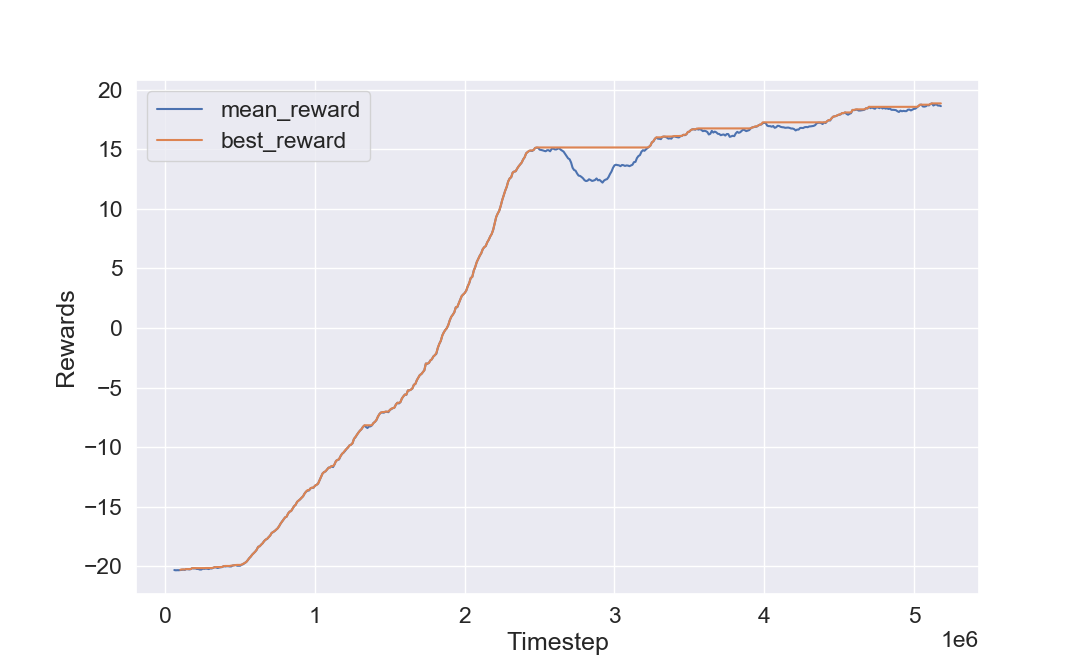
\includegraphics[height=3.4in]{part1_q1.png}
  \caption{Learning curves for basic Q-learning on game Pong}
\end{figure}
\begin{lstlisting}[language=bash]
python run_dqn_atari.py
\end{lstlisting}

\subsection*{Question 2: double Q-learning}
\begin{figure}[H]
  \centering
  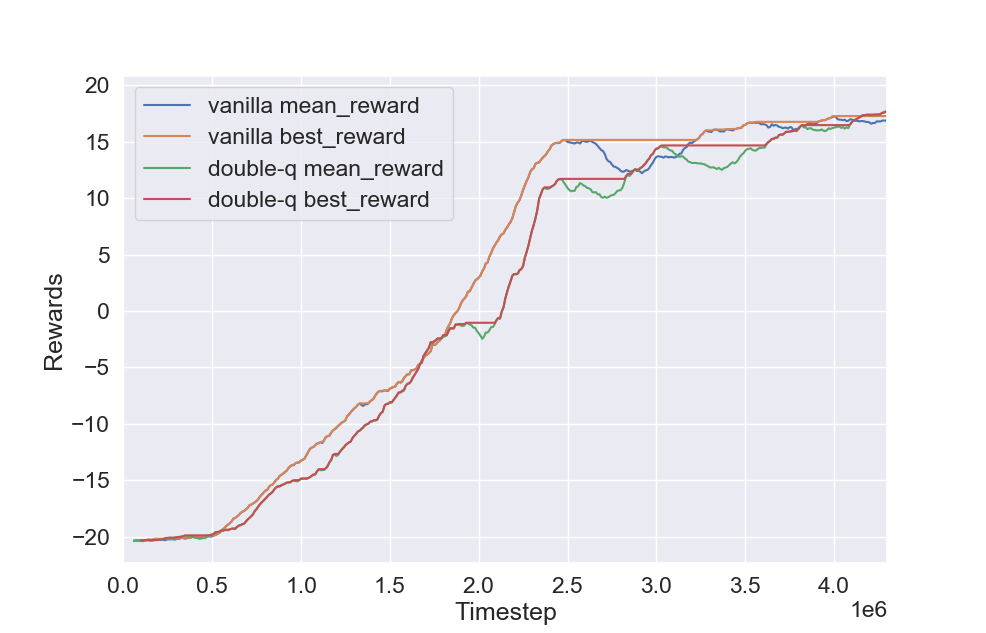
\includegraphics[height=3.4in]{part1_q2.png}
  \caption{Learning curves for vanilla vs double Q-learning on game Pong}
\end{figure}
\begin{lstlisting}[language=bash]
# manually change line 87 in run_dqn_atari.py to pass double_q=True
python run_dqn_atari.py
\end{lstlisting}
We can see that both vanilla and double Q-learning reach to rewards 15+ after 4M timesteps. The double Q-learning is slightly better than vanilla at 4M timesteps. This matches the Figure 4 of \href{https://arxiv.org/pdf/1509.06461.pdf}{this paper}. Also noticed that the learning curve is little slow for double Q-learning, however this probably because of the random seed.

\subsection*{Question 3: experimenting with hyperparameters}
\begin{figure}[H]
  \centering
  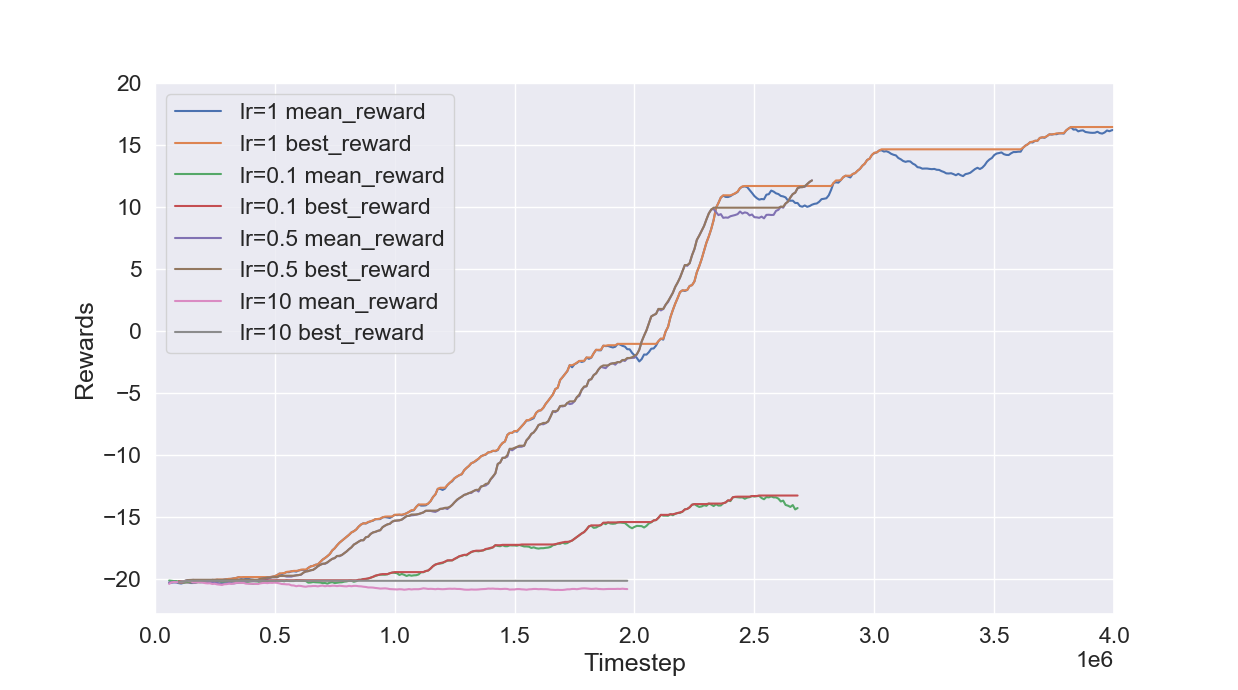
\includegraphics[height=3.4in]{part1_q3.png}
  \caption{Learning curves of \textit{learning rate multiplier=0.1, 0.5, 1, 10} on game Pong with double Q-learning}
\end{figure}
\begin{lstlisting}[language=bash]
# manually change line 87 in run_dqn_atari.py to pass double_q=True
python3 run_dqn_atari.py 0.1 
python3 run_dqn_atari.py 0.5
python3 run_dqn_atari.py 10
\end{lstlisting}
Here we choose the \textit{learning rate multiplier} to experiment with the hyper-parameters.
We can see that with learning rate very large the Q-learning basically can not learn anything, the rewards of lr=10 did not increase after 2M timesteps. The curve of lr=0.1 is actually increasing, but slowly, it probably will get the high rewards, but will take more time. The performance of lr=0.5 is very much similar to lr=1.

\newpage
\section*{Part2 Actor-Critic}

\subsection*{Question 1: Sanity check with Cartpole}
\begin{figure}[H]
  \centering
  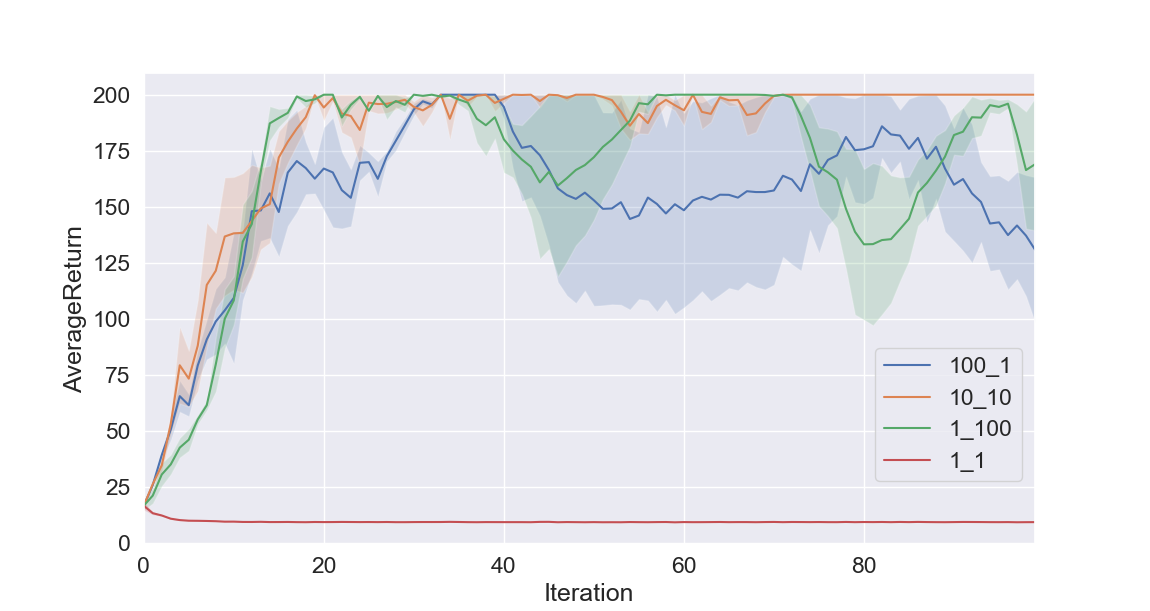
\includegraphics[height=3.4in]{part2_q1.png}
  \caption{Learning curves of different number of target updates and number of gradient combinations on CartPole with Actor-Critic. We can see that (ntu=10, ngsptu=10) is best parameter combination, as it converges to the optimal rewards fast and more stable than (1, 100).}
\end{figure}
\textbf{Explanation}: Since we are using neural network to fit value function, (ntu=1, ngsptu=100) means we only update target once, while taking many gradient descent steps. This will probably bring network too close to the current target, instead of fitting to get a more generalized value function. The bias will be larger compared with (ntu=10, ngsptu=10). For (ntu=100, ngsptu=1), we only take one gradient step, so it is likely that we will not have chance to fit value function, and finally get larger bias.


\newpage
\subsection*{Question 2: Run actor-critic with more difficult tasks}
We can see that the performance is similar to what we got in HW2, but slightly worse.
\begin{figure}[H]
  \centering
  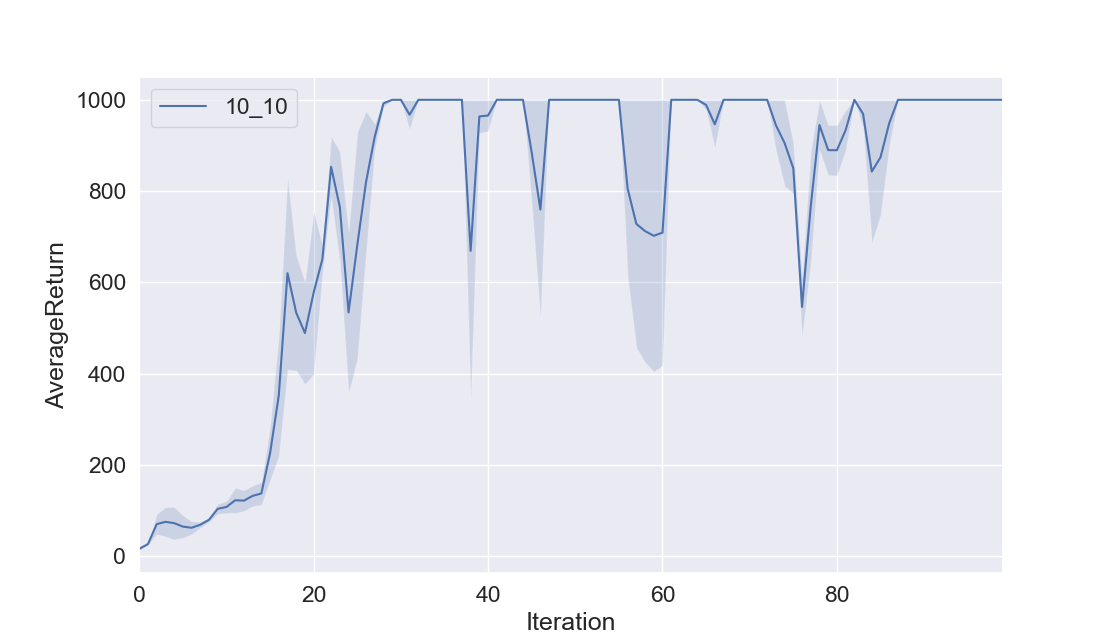
\includegraphics[height=3.4in]{part2_q2_2.png}
  \caption{Learning curves of InvertedPendulum with ntu=10 and ngsptu=10}
\end{figure}
\begin{lstlisting}[language=bash]
python train_ac_f18.py InvertedPendulum-v2 -ep 1000 --discount 0.95 -n 100 -e 3 -l 2 -s 64 -b 5000 -lr 0.01 -clr 0.01 --exp_name 10_10 -ntu 10 -ngsptu 10
\end{lstlisting}
\begin{figure}[H]
  \centering
  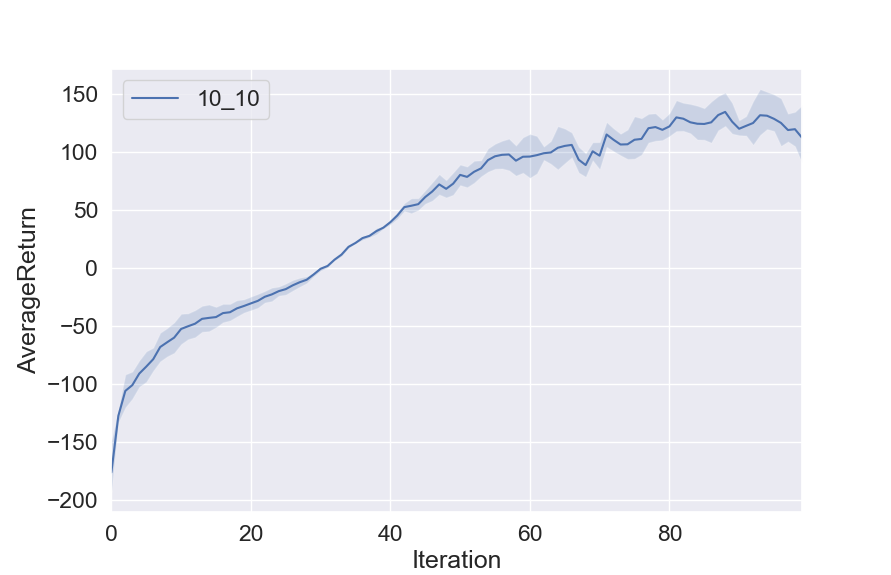
\includegraphics[height=3.4in]{part2_q2_1.png}
  \caption{Learning curves of HalfCheetah with ntu=10 and ngsptu=10}
\end{figure}
\begin{lstlisting}[language=bash]
python train_ac_f18.py HalfCheetah-v2 -ep 150 --discount 0.90 -n 100 -e 3 -l 2 -s 32 -b 30000 -lr 0.02 -clr 0.02 --exp_name 10_10 -ntu 10 -ngsptu 10
\end{lstlisting}

\newpage
\subsection*{Bonus}
Here I am trying to tune actor-critic such that it could perform better.
\begin{enumerate}
\item Add 2 more hidden layers for critic network.
\item Use separate smaller learning rate to train critic network (0.01, 0.001).
\item Increase the number of target updates to 20.
\end{enumerate}
From the Figure 7, we can see that after tunning, the performance is getting better, and is very similar to what we got in HW2. The best one has critic\_learning\_rate=0.01, ntu=20, ngsptu=10, and this also has lower variance.
\begin{figure}[H]
  \centering
  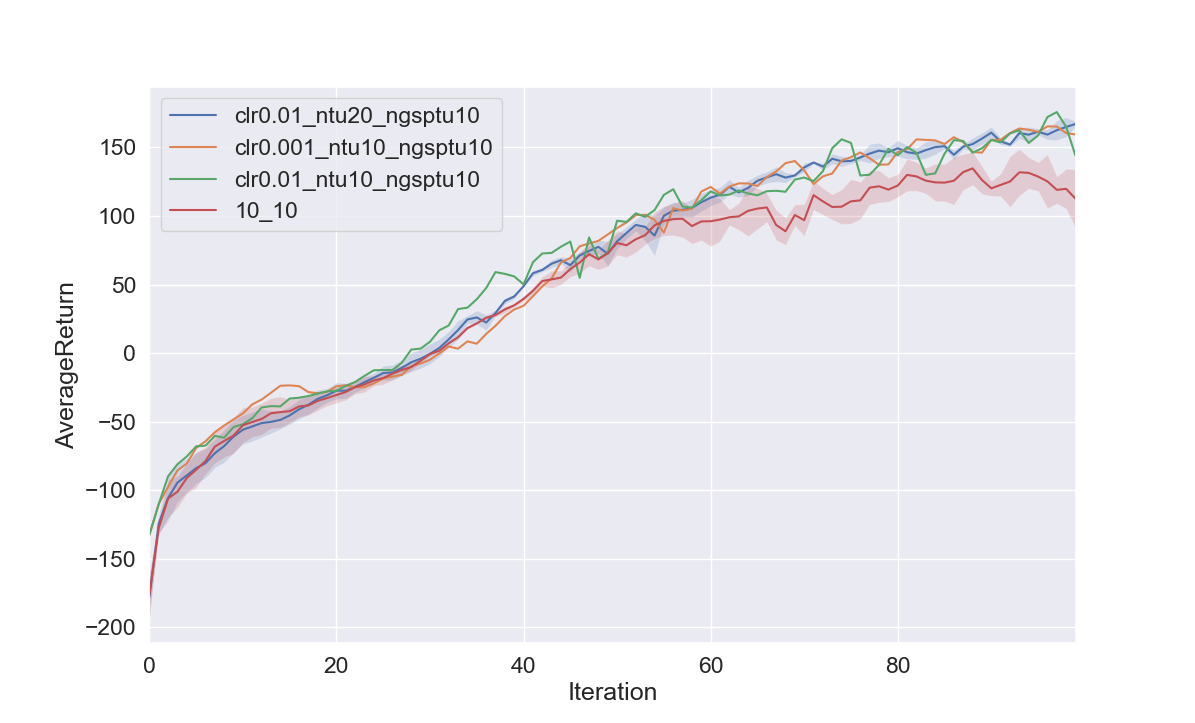
\includegraphics[height=3.4in]{bonus.png}
  \caption{Learning curves of HalfCheetah. \textit{clr} is representing critic-learning-rate.}
\end{figure}
\begin{lstlisting}[language=bash]
# please change line 263 in train_ac_f18.py to use "n_layers=self.n_layers + 2" before running
python train_ac_f18.py HalfCheetah-v2 -ep 150 --discount 0.90 -n 100 -e 3 -l 2 -s 32 -b 30000 -lr 0.02 -clr 0.01 --exp_name clr0.01_ntu10_ngsptu10 -ntu 10 -ngsptu 10
python train_ac_f18.py HalfCheetah-v2 -ep 150 --discount 0.90 -n 100 -e 3 -l 2 -s 32 -b 30000 -lr 0.02 -clr 0.001 --exp_name clr0.001_ntu10_ngsptu10 -ntu 10 -ngsptu 10
python train_ac_f18.py HalfCheetah-v2 -ep 150 --discount 0.90 -n 100 -e 3 -l 2 -s 32 -b 30000 -lr 0.02 -clr 0.01 --exp_name clr0.01_ntu20_ngsptu10 -ntu 20 -ngsptu 10
\end{lstlisting}


\end{document}













